\section{BJT in Saturation Mode}
Change the value of \textbf{R1 to 1k} and run the simulation again. Capture the simulation results and explain the values of $I_B, I_C, V_{CE}$. The default transistor gain is $\beta = 100$, and the saturated voltage $V_{CE(Sat)} = 0.65V$ and $V_{BE} = 0.7V$.

\begin{figure}[!htbp]
    \centering
    \textbf{Your image goes here:}
    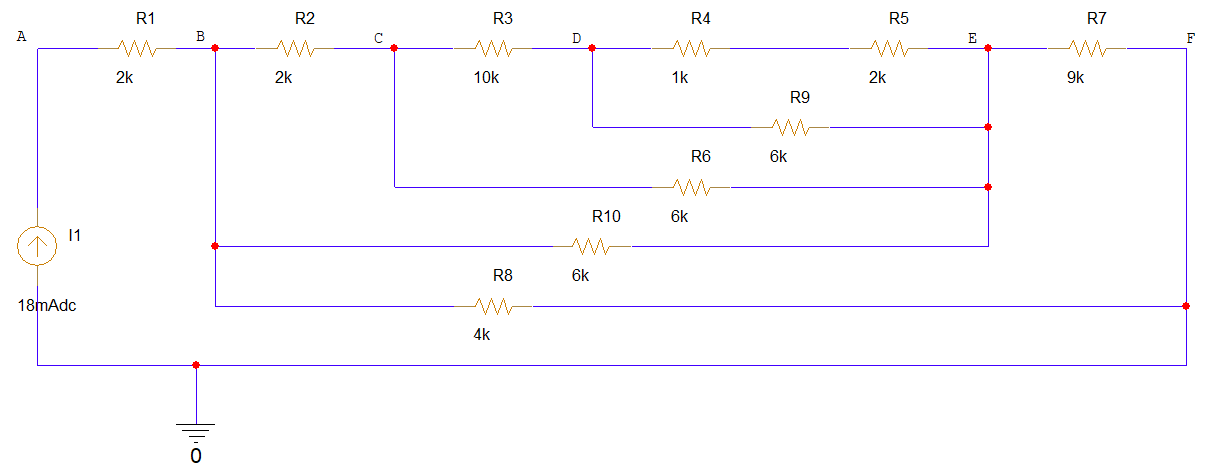
\includegraphics[width=0.8\linewidth]{graphics/ex1/f1.PNG}
    % \vspace{6cm}
\end{figure}
Kết quả trong PSpice được giải thích như sau:

\begin{itemize}
    \item Áp dụng định luật Ohm, $I_B = \frac{V_{BB} - V_{BE}}{R_1} = \frac{5V - 0.7V}{1000\Omega} =  4.3$ mA
    \item Giả sử transistor ở vùng tích cực, $I_C = \beta \times I_B = 100  \times 4.3mA = 0. 43$ A  
    \item Cuối cùng, để kiểm chứng giả định trên $$V_{CE} = V_{CC} - I_C \times R_2 = 10V - 0.43A \times 100\Omega = -32V$$
\end{itemize}

Vì $V_{CE} < 0$, giả định trên là sai. Transistor đang ở vùng bão hòa. Do đó, $I_C$ được xác định như sau:\\

$$I_C = \frac{V_{CC} - V_{CE(Sat)}}{R_2} = \frac{10 - 0.65}{100} = 93.5 mA$$

